\section*{Appendix}\label{appendix}

\setcounter{page}{1}

\subsection{Network Architectures}
The following section includes graphical representations of NN referenced throughout the thesis. %TODO: briefly describe the kindf of archs shown in this section...

\subsubsection{Classifiers}\label{appendix_classifiers}
TODO: the caption of the classifiers needs to be adjusted to account for the fact that these are also used to run the stratifiedclassifiers task. 
The graphical representations of the network architectures are created with the tool \textit{visual keras}, by Paul Gavrikov (\cite{Gavrikov2020VisualKeras}).

\begin{figure}[htbp]
    \centering
    \vspace{-.5em}
    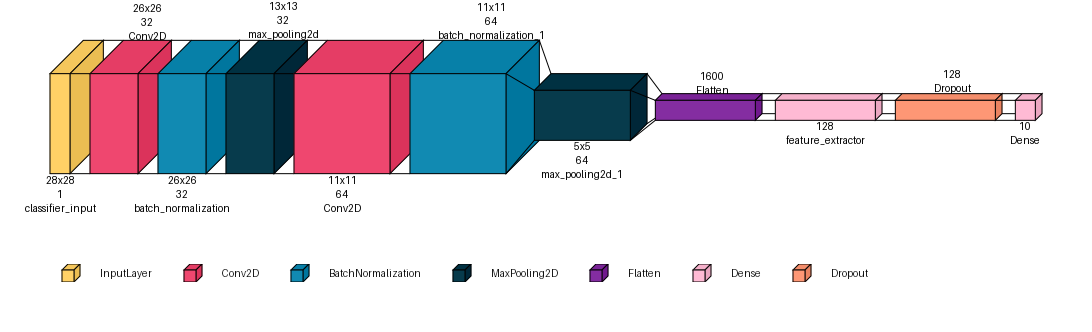
\includegraphics[width=.9\textwidth]{abb/netron_network_archs/classifying_Classifier_MNIST.png}
    \caption{Depiction of the CNN achritecture used to classify unlabeled images from the MNIST GDA experiments. (Image created with \cite{Gavrikov2020VisualKeras})}
    \label{fig:figure_class_mnist}
\end{figure}

\begin{figure}[htbp]
    \centering
    \vspace{-2em}
    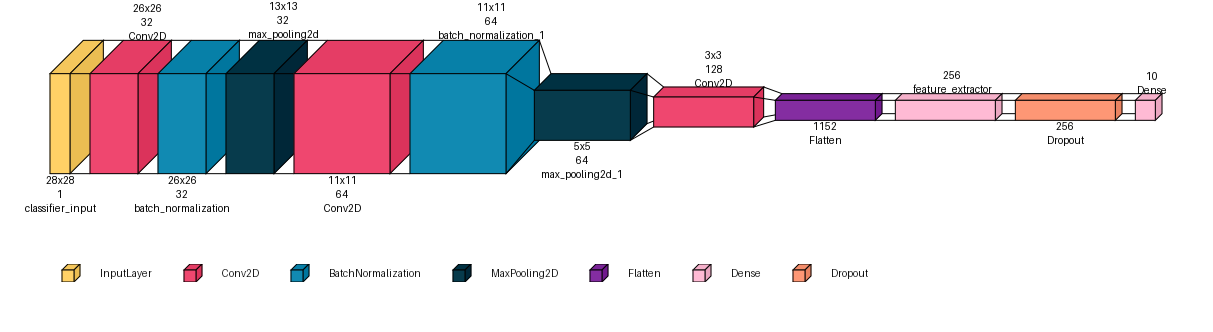
\includegraphics[width=.9\textwidth]{abb/netron_network_archs/classifying_Classifier_FashionMNIST.png}
    \caption{Depiction of the CNN achritecture used to classify unlabeled images from the FashionMNIST GDA experiments. (Image created with \cite{Gavrikov2020VisualKeras})}
    \label{fig:figure_class_fashion}
\end{figure}

\begin{figure}[htbp]
    \centering
    \vspace{-2em}
    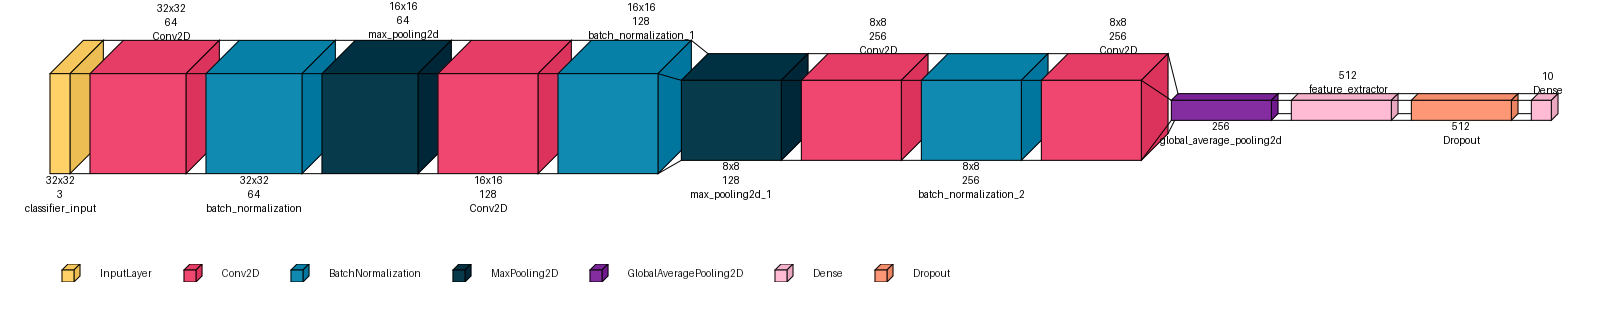
\includegraphics[width=.9\textwidth]{abb/netron_network_archs/classifying_Classifier_Cifar10.png}
    \caption{Depiction of the CNN achritecture used to classify unlabeled images from the CIFAR10 GDA experiments. (Image created with )}
    \label{fig:figure_class_cifar10}
\end{figure}